\chapter{Design}
\label{design}
\section{Program Requirements}
\label{programRequirements}

\subsection{Motivation}
While the detriments to SAON technologies are well-known \cite{Akbarzadeh2013}, \cite{Heupel2006}, \cite{Howard2002},  \cite{Kessel2015}, \cite{Steel2014} there few tools/services to analytically design SAONs around them.  Further, none of these tools/services are free and open-source.


\subsubsection{Cost Efficiency}
\label{motivationCost}
In section~\ref{CostAltTech}, we discuss the costs of marine telemetry systems, noting that acoustic telemetry systems produce data at a significantly lower ($\ge$10x cheaper) cost than VHF or GPS/Satellite based technologies.  In order to maintain the cost-efficiency of acoustic technology, at least 10$\%$ of the produced transmissions must be captured by the SAON's receiver array.  Given the numerous (but avoidable) impediments to reception of these acoustic signals (\ref{RulesOfThumb}), the array-design process becomes critical to maintaining the cost-efficiency of SAON technologies.  A free network design tool would help to maintain the cost-efficiency of SAONs by eliminating costs surrounding their design and evaluation.  


\subsubsection{Metrics}
\label{motivationMetrics}
The computation of network metrics (Absolutes Recovery Rate, Unique Recovery Rate, Network Sparsity) is very labor intensive at large scale.  Additionally, the process of computation may vary from experiment to experiment.  An automated tool would solve both issues by providing a fast, simple, repeatable, and well-documented method for computation.  Metrics from such a tool would be useful in directly comparing different network deigns.


\subsubsection{Transparency}
\label{motivationTransparency}
An open-sourced tool/service would make the design process more transparent, permitting peer-review and modification.  This would provide increased confidence in the process, and increased adoption of the tool.  Increased adoption would result in a larger number of efficient SAONs, leading to higher data recovery rates, better data quality, increased return-on-investment, and the ability to better address scientific-research questions.


\subsection{Supported Workflows}
\label{workflows}
\subsubsection{Static Analysis}
\label{staticAnalysis}
As mentioned in section~\ref{motivationMetrics}, a primary motive for this tool was the ability to create a repeatable means of measuring the performance of a SAON.  To this end, the ability to measure an existing network design is important.  Users should be presented with network metrics after specifying bathymetry, receiver locations, network properties, and an animal model for a given study site.


\subsubsection{Optimal Design}
\label{optimalDesign}
The primary motive for this tool is the ability to design optimal SAONs.  Users should be presented with a network design (optimal receiver locations), and network metrics after specifying bathymetry, the number of receivers in the network, network properties, and an animal model for a given study site.


\subsubsection{Optimal Addition}
\label{optimalAddition}
Similar to the problem of optimal design, is the problem of optimal addition: the augmentation of an already existing SAON.  Users should be presented with a network design (optimal augmenting receiver locations), and network metrics after specifying bathymetry, the number of receivers to add to the network, network properties, existing receiver locations, and an animal model for a given study site.

\section{Conceptual Model}
\label{conceptualModel}
\subsection{Time/Space Modeling}
\label{timeSpaceModel}
\subsubsection{Spatial Modeling}
\label{spatialModeling}
To model a 4-dimensional underwater environment (a 3-dimensional spatial grid of various attributes), we use a two-dimensional grid of cells (in the x and y dimensions) containing numerical values.  Numerical values in those cells, combined with other user-defined values, can then be used in various shape functions to generate a third dimension (z) of values for that cell.  In this way, we save significant amounts of memory by computing values for a specific three-dimensional cell on the fly, instead of storing an additional dimension of values.  

\subsubsection{Temporal Modeling}
\label{temporalModeling}
With respect to the passage of time, our model assumes that receivers are stationary throughout the entire experiment.  Furthermore, the animal model does not represent animal movement over time, but the percentage of time an animal would spend in a particular cell over the entire study period.  The animal model therefore represents the tendency of an animal's movements over the expected study period rather than its particular movements in a small time period.  As a result, we need not consider temporally-related phenomena. 




\subsection{Bathymetric Modeling}
\label{bathymetyricModeling}
\subsubsection{Bathymetric Grid}
\label{bathymetricGrid}
Bathymetry files are generally given as two-dimensional matrix of numerical values or a list of x,y,z values.  Bathymetric files describe a three-dimensional space as a regular grid of rectangular prisms (cells) with constant length (x-dimension) and width (y-dimension), but varying negative (depth is negative)  heights (z-dimension).  The resolution of a bathymetric file is given by the x and y (length and width) dimensions of its cells.  For example, a 50 meter Bathymetry file has cell sizes of approximately 50 meters square (although these cells are not necessarily perfectly square).  Bathymetric files list beginning and ending coordinates (North/South Latitudes and East/West Longitudes), as well as the grid size (in rows and columns) in cells.  With these two measurements, one can compute the degrees per cell of latitude and longitude.  Thus, particular latitudes and longitudes can be converted to rows/columns, and back.  

Our program works on a two-dimensional, grid-based system, taking advantage of the grid given by the user-provided bathymetric file.  As stated in section~\ref{spatialModeling}, the bathymetric grid is a grid containing numerical values that describe a third dimension (depth).  The exact spatial extent of this description is given by the bathymetric file.  Thus, the resolution of our program's output is dictated by the resolution of the input bathymetric file. 

\subsubsection{Bathymetric Filetypes}
Two highly popular file formats in Geographical Information Systems are provided by NetCDF and ArcGIS.  NetCDF provides an open source file format that lists a header of metadata and a white-space delimited matrix of numerical values.  ArcGIS is a private institution that supplies many different file types, formats, and encodings for a family of GIS-related software systems.  ArcGIS also supports the encoding and transcription of its proprietary formats to the NetCDF format.  Due to the large number of possible format and encoding combinations in ArcGIS file formats and the ability to translate file these various formats to NetCDF, we natively support the NetCDF standard, and assume that users are capable of converting their data into the NetCDF format.  


\subsubsection{Bathymetric Resolution}
Two key components of our program are the animal model and the bathymetric shadowing model.  These models make decisions based upon the depth at a particular cell and the distance between cells, data which is governed by the input bathymetry file.  As stated in Section~\ref{bathymetricGrid}, the resolution of the program's output is dependant upon the resolution of the input bathymetry file.  Obviously, higher resolution grids will offer higher resolution results; but, high-resolution bathymetric files tend to be difficult to come by.  These files are often held by private agencies, or simply never released to the public.  It may then seem useful to artificially increase the resolution of the simulation by dividing the input file's bathymetric cells into sub-cells of finer resolution, but doing so increases the computational size of the program without meaningfully increasing the accuracy of the results.    
 
 
When subdividing cells, either the sub-cells are given the same depth as their parent cell, or the depth of a sub-cell is interpolated from surrounding cells by some smoothing function.  Subdividing a cell into sub-cells with the same depth makes the assumption that all sub-cells are actually the same depth.  Furthermore, this results in the animal and bathymetric shadowing models making the same depth-based decision for all sub-cells that they would for the larger parent cell, increasing the computational load (see Figure~\ref{duplicate}).  Subdividing a cell into sub-cells with a depth governed by a smoothing function makes the assumption that there are no impeding obstacles between neighboring cells, and that there is a smooth transition between them (see figure~\ref{smooth}).  Subdividing the two cells in Figure~\ref{LoS} half (ignoring for now the y component of our grid) results in the four sub-cells with depths given by a smoothing function (Figure~\ref{smooth}) would result in the large depth change at the sheer cliff face in Figure~\ref{LoS} being smoothed into smaller changes in depth, which would allow the unobstructed transmission of acoustic signals.


Both strategies (duplicating depth and applying a smoothing function) for artificially increasing the resolution of a bathymetric file disregard the manner in which the bathymetry was originally observed.  Bathymetry is almost always computed as the average observed depth at several points within a geographic area of a given size (resolution).  For example, imagine a particular cell in a bathymetric grid has a steep cliff running across the middle.  Assuming that the sea floor at the top and base of the cliff were perfectly flat, and one measurement was taken at the top of the cliff and one at the bottom, the cell would have a depth equal to the average of the two observed depths.  This average depth would then represent the depth for that entire cell, modeling it as a perfectly flat surface.  Obviously this is problematic as the true nature of the sea floor is misrepresented.  This misrepresentation leads to two conflicting arguments, the first is that the application of smoothing functions or duplicating depths of already averaged data makes faulty assumptions about real-world bathymetry.  On the other hand, because source bathymetric files already represent aggregate data, one could argue that any conclusions drawn from the source bathymetry files are already faulty.  We argue that the conclusions one can make are only as good as the bathymetric information available.  As the resolution of measured bathymetry (bathymetric measurements taken from the real world) increases (becomes finer), so too does the accuracy of the simulation.  While artificially increasing the resolution of a source bathymetric file may skew results, it is sometimes useful for meshing two bathymetric source files of varying resolution into one larger bathymetric dataset.  Our program does not currently support modifying the resolution of source bathymetric files.


\begin{figure}[h]
	\label{resolutionScale}
	\begin{subfigure}{.5\textwidth}
		\centering
		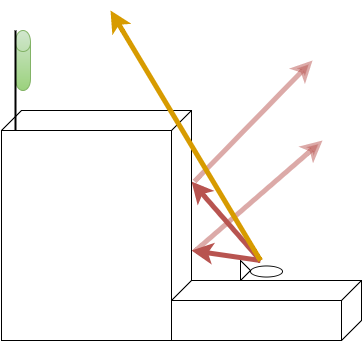
\includegraphics[width=.8\linewidth]{LoS.png}
		\caption{}
		\label{LoS}
	\end{subfigure}%
	\begin{subfigure}{.5\textwidth}
		\centering
		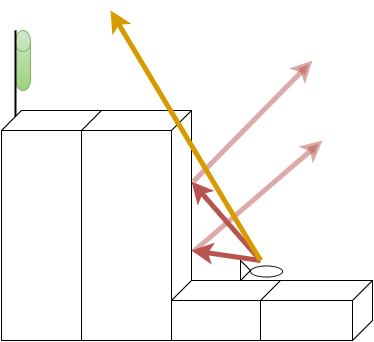
\includegraphics[width=.8\linewidth]{duplicate.png}
		\caption{}
		\label{duplicate}
	\end{subfigure}
	\begin{subfigure}{.5\textwidth}
		\centering
		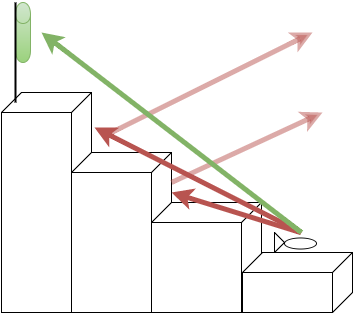
\includegraphics[width=.8\linewidth]{smooth.png}
		\caption{}
		\label{smooth}
	\end{subfigure}
	
	\caption{(a) illustrates the bathymetric shadowing model for two adjacent cells within a bathymetric grid.  (b) shows how artifically increasing the resolution of the bathymetric grid form (a) using the duplication method of cell sub-division does not affect the bathymetric shadowing model, but increases the number of cells to consider.  (c) shows how artificially increasing the resolution using a smoothing function increased the number of cells to consider and can lead to inflated signal reception.}
\end{figure}


\subsubsection{Bathymetric Shadowing}
\label{bathymetricShadowing}
In the real world, the transmission of an acoustic ping originates from the tagged animal and propagates to the receiver.  This propagation is governed by complex interactions with the surrounding environment (including the bottom substrate, water density, distance to the surface/sea-floor, thermoclines, the number of tagged animals in the vicinity, and ambient noise).  Because it is difficult to model these phenomena without significant data on a large number of variables over a large area, our simulation uses a simplified propagation model relying on direct line of sight between a tagged animal and a receiver.  Simply put, in order to receive a transmission, there must exist a physically-unobstructed path between a tagged animal and a receiver.  




\subsection{Animal Modeling}
\label{animalModeling}

\subsubsection{Behavior Grid}
\label{behaviorGrid}
Animals exhibit many different movement patterns and habitat preferences (both of which can vary in three-dimensional space).  This greatly affects their distribution within the study space, and thus the network configuration that should be deployed to capture their movement.  To describe the distribution of transmissions released from tagged animals, we utilize a two dimensional grid of the same dimensions and resolution as the Bathymetry Grid (Section~\ref{bathymetricGrid}).  Each cell in this "Behavior Grid" contains a positive real value indicating, out of all transmissions that will be released over the entire experiment period, the percentage of transmissions that are expected to be released from within that cell's water column.  This value can loosely be though of as the "animal-residency" of a cell since we are effectively measuring the number of animal-hours spent in that cell.  

To populate this 2D grid with values, we provide two behavioral models to simulate the horizontal distribution of animals, and two optional models for the vertical distribution.  Note: we use the terms "animal" and "transmission" interchangeably as we are interested in capturing acoustic transmissions, which are given off by the tags carried by the target species.  


\subsubsection{Animal Movement Modeling}
\label{animalMovementModel}
To simulate tagged animal movement across the two dimensional x/y space (as one would expect to see on a map from above), we provide two basic probabilistic movement models: Random Walk, and Ornstein-Uhlenbeck(OU).  

\paragraph{Random Walk Model}
\label{randomWalkModel}
The Random Walk model assumes that animals move randomly through the environment.  As a result, over the entire study period, each valid grid cell (as defined by the Restricted Vertical Habitat Range (Section~\ref{restrictedVerticalHabitat})) will see an equal amount of animal traffic.  The result is that every valid cell  in the grid will have the same chance of capturing an animal's acoustic transmission.  We assume that tagged individuals will be willing and able to very briefly (in probabilistically negligible time frames) pass through inhospitable (over dry land, through impassible terrain) cells to get to other cells.  This means that disjoint sections of habitat are still equally likely to see animal presence.

\paragraph{Ornstein-Uhlenbeck Model}
\label{ouModel}
The Ornstein-Uhlenbeck(OU) model\cite{OU} supports the idea that over time, animals will tend to congregate near certain points of interest.  This concept models an animal's desire to seek out and remain near a physically significant structure, a region of high food availability, breeding grounds, shelter, etc.  The OU algorithm allows for the modeling of the attraction towards a focal point in the x/y directions separately.  Assuming a center point at the origin of a Cartesian grid, increasing the attraction in the x-direction will bring the distribution closer to the x-axis, and decreasing it will spread the distribution away from the x-axis.  A correlation value ($-1\le x \le 1$) allows for tilting the angle of the distribution.  A positive correlation value tilts the distribution clockwise, and a negative correlation value tilts it counter clockwise.  Correlations of 0 (no tilt), 1 ($180^{\circ}$ tilt), and -1 (-$180^{\circ}$ tilt) will have no observable effect on the distribution.


\begin{figure}[h]
	\label{OUimg}
	\centering
	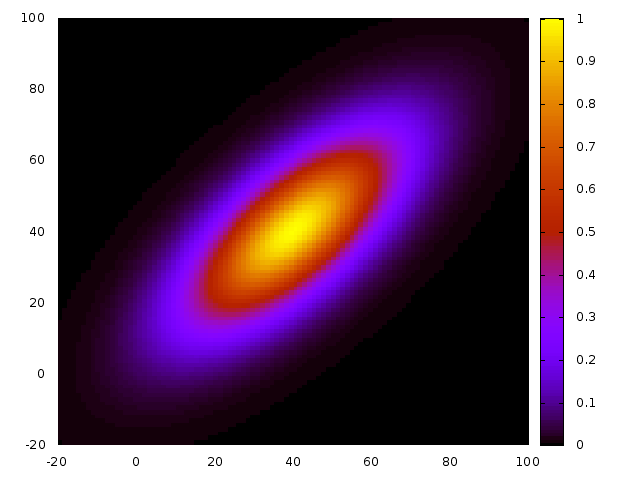
\includegraphics[scale=0.5]{OUpos7.png}
	\caption{An example of a distribution given by the Ornstein-Uhlenbeck Model with a high attraction value in the x-direction, a low attraction value in the y-direction, and a correlation value of 0.7.}
\end{figure}


\subsubsection{Habitat Preference}
\label{habitatPref}
Some animals exhibit the preference to reside within a specific section of the water column; for example, prey animals may prefer hiding in reef heads at the bottom of the water column, while predators will prefer to hover several meters off the bottom.  This preference can be incorporated into the animal model by specifying mean (preferred Depth") and standard deviation("SD of Preferred Depth") values.  These values are given as a measure of the distance (in meters) from the bottom.  For example, specifying a depth of '0' for Preferred Depth indicates that the animal prefers to live on the sea floor, while a value of '5' indicates that the animal prefers to live 5m off the sea floor.  Allowing a standard deviation value allows for the modeling of animals that tend to be sedentary within the water column (a small deviation), and those that migrate through the water column (a large deviation).  Currently, the simulation does not support the modeling of sub-surface animals, and any part of the distribution curve falling below the sea floor will be redistributed along the rest of the curve. 


\subsubsection{Restricted Vertical Habitat Range}
\label{restrictedVerticalHabitat}
Some animals will live only in a specific depth range.  For example, a deep sea fish may live only in depths of 300-400 meters.  To incorporate this into the behavioral model, users can specify a minimum and maximum vertical habitat range for their animal.  If this option is selected, the program will only simulate animals in cells whose maximum depths are between the given minimum and maximum depths.  As in the Random Walk Model, we assume that animals are willing and able to move between disjoint areas of habitat.


\subsection{Receiver Modeling}
\label{receiverModel}

\subsubsection{Acoustic Attenuation}
\label{acousticAttenuation}
As acoustic transmissions travel away from their point of origin, they experience significant attenuation.  We model this attenuation of acoustic signal as a deteriorating function following a Gaussian distribution.  Given a particular distance between a tag and receiver, this distribution describes the probability of capturing the transmission.  Depending upon the environment, the highest probability of detection generally occurs a few meters away from the receiver.

\subsubsection{Detection Range}
\label{detectionRange}
The distance at which a transmission from an acoustic tag can be captured is largely determined by the transmission power of the acoustic tag.  In our model, we assume that all animals have the same model of acoustic tag, and that "transmission range" is instead a property of the receiver referred to as "Detection Range" ($D_{range}$).  We define the Detection Range of a receiver to be the average distance (specific to the given study site) at which the probability of detection drops to 5\%.

\subsubsection{Detection Area}
\label{detectionArea}
We define the Detection Area of a receiver to be the square plane of grid cells around a receiver which will be considered when evaluating a potential receiver emplacement.  Theoretically, the Detection Area of a receiver is a circle with a radius equal to the receiver's Detection Range ($D_{range}$).  Within our program, we model the Detection Area as a square grid of cells with an edge length equal to 2*$D_{range}$ + 1, centered on the cell where a receiver will theoretically be placed.  The additional cell ensures odd dimensions for the square, so that there exists a central cell to model as the receiver.  We model a square instead of a circle for simplicity of book keeping (we simply keep track of the Detection Range, and starting row/column indexes).  The theoretical Detection Range can then be imagined as a circle circumscribed in the square of our model.  At first glance, it might seem that this simplification would alter the probabilistic distribution models as additional "gray" cells (those outside the circle but within the square) are being considered.  However, this is not the case as those models utilize exponential functions based on the absolute distance from the receiver.  Gray cells will therefore contribute exponentially less to the total probability than those cells within the Detection Range, and their effect on the final probability will be negligible.  

\subsubsection{Network Specification}
There are three distinct ways to place receivers into the model: user specification, optimal placement, and optimal projection.  User Specified Receivers (USR) represent receivers that are already deployed at the study site and are being integrated into a larger network.    Program Placed Receivers (PPRs) are receivers that will be  optimally placed by the program, taking into account existing (user specified) receivers placements using the suppression dynamic explained in section~\ref{suppression}.  Projected Receivers are PPRs that do not count towards the network statistic rates returned by the program.  Instead, their contributed recovery rates are given separately, and represent the marginal benefits of incrementally placing more receivers.  


\section{Evaluation of Receiver Emplacements}
\label{evaluationOfReceiver}
Section~\ref{animalModeling} discusses the models used to simulate animal movement.  These animal models populate the "Behavior Grid", a 2D grid (of the same size as the specified bathymetry grid) which gives the distribution of animals across the study area, and a shape function which describes a normal distribution of animals within the water column at various depths.  Section~\ref{LoS} discusses the Line of Sight (LoS) model used to simulate the obstruction of acoustic transmission.  Section\ref{receiverModel} discusses how attenuation affects the propagation of acoustic signals and thus the probability of detecting ($P_{range}$) acoustic transmissions from a distance.  Together, these models are used to evaluate receiver locations throughout the study site.  


\subsection{Goodness Grid}
\label{goodnessGrid}
In modeling our 3D environment (the study site), we make extensive use of 2D grids with a third dimension.  However, we assume all receivers in the study will have the same elevation off the sea floor.  Recall that our program will evaluate every cell in the Bathymetry Grid as a potential receiver emplacement.  Together with the assumption of fixed receiver elevation, the search space considered by our program is a 2D surface parallel to the sea floor.  Thus, it makes sense to store the evaluation metric for this search space in a 2D grid with the same dimensions and resolution as the Bathymetry Grid.  This gird is referred to as the "Goodness Grid" ($G$).  

\subsection{Evaluation Algorithms (Bias)}
The Evaluation or “Goodness” algorithm is the driving force behind the evaluation of receiver placements.  Given a particular cell at row i and column j, an Evaluation Algorithm will compute a non-negative, rational value representing how much data a receiver placed d meters off the bottom of cell (i,j) would recover, according to the particular bias of a given evaluation algorithm.  These values are computed for all cells within the Bathymetry Grid, and stored in the Goodness Grid.  $G_{i,j}$ refers to the goodness value of the cell at row i, column j on the Goodness Grid($G$).  

While users are able to write their own “Goodness” algorithms, three basic algorithms are provided.  All Evaluation Algorithms compute the goodness of a potential receiver location ($G_{i,j}$) by summing the number of Estimated Receivable Transmissions (ERT) from all cells within Detection Range of $G_{i,j}$ .  Each algorithm has a particular bias in its approach to computing ERT.  Note: we utilize the terms "bias" and "algorithm" interchangeably when referring to "Evaluation Algorithms".\newline
\newline
Explicitly, $G_{i,j} = \Sigma_{i=i_0}^{i_n} \Sigma_{j=j_0}^{j_n} ERT(x,i,j)$, where x is the chosen Evaluation Algorithm/Bias, $i_0$ and $j_0$ represent starting row/column indexes (respectively) for the Detection Area, and $i_n$ and $j_n$ represent ending row/column indexes (respectively) for the Detection Area.  Given that the Detection Area is of size $(2*D_{range}+1)^2$, the expected computation time of evaluating

\subsubsection{Animal Only (Option “1”)}
\label{bias1}
This option prefers to place receivers in areas of high animal activity, completely oblivious to the surrounding bathymetry.  This is useful for when no bathymetric information is available or when animal activity occurs well above the sea floor.   The "Animal Only" option computes ERT for a cell as the animal-residency of a cell (according to the Behavior Grid), multiplied by the probability of detection due to attenuation for that cell's distance from the receiver.\newline
Explicitly,
$ERT_{1,i,j} = B_{i,j} * P_{Attenuation}(Range(i,j))$

\subsubsection{Visible Fish (Option “3”)}
\label{bias3}
This option chooses receiver locations that have the best view of areas of high animal residency.  Both animal presence and visibility due to topography are considered. This option is most useful when both well-documented animal behavior and high resolution bathymetry are available.  ERT is computed as animal-residency (according to the Behavior Grid), multiplied by the percentage of visible fish (given either as a simple percentage of the visible water column, or by integration over the shape function described in Habitat Preference), multiplied by the probability of detection due to attenuation.  Figure~\ref{observableAnimals} depicts this operation.\newline
Explicitly,
$ERT_{3,i,j} =  B_{i,j} * P_{observation} * P_{Attenuation}(Range(i,j))$

\begin{figure}[h]
	\label{observableAnimals}
	\centering
	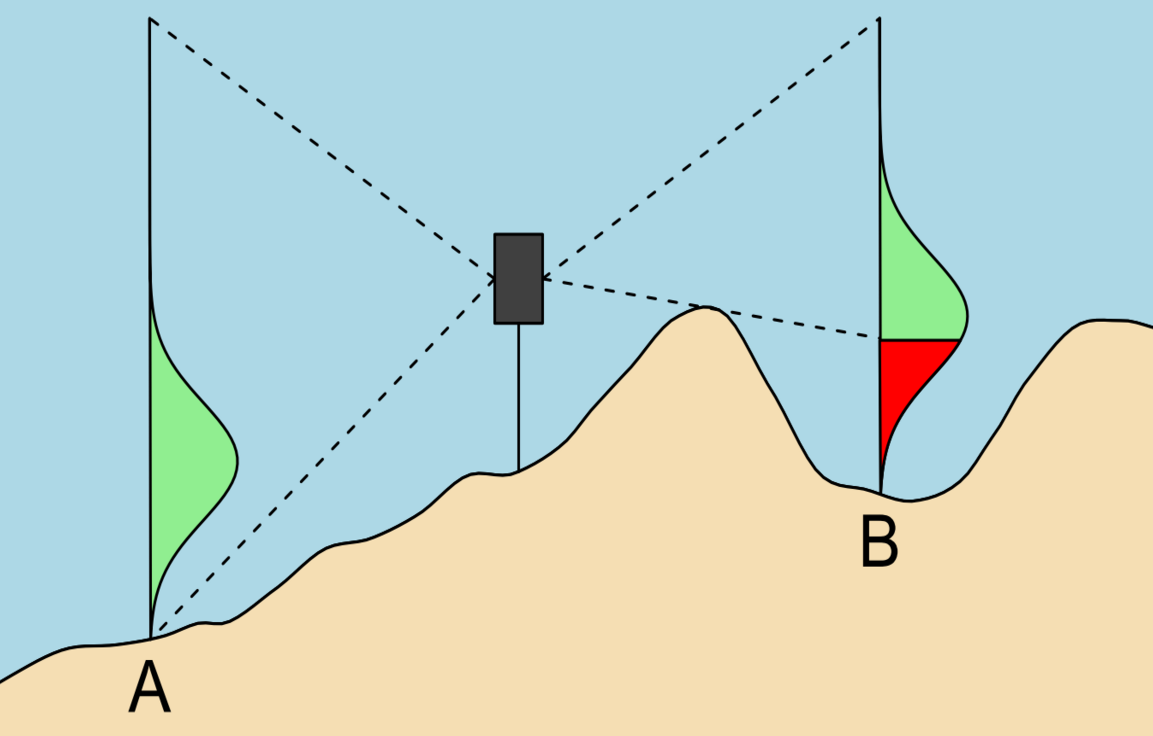
\includegraphics[scale=0.3]{ObservableAnimals.png}
	\caption{An illustration of how ray tracing and integration over a shape function can be used in Option 2 \& Option 3 to compute the probability of detecting fish within a cell.  Dotted lines indicate the maximum and minimum depths visible to the receiver.  The normal distributions in green/red indicate the distribution of fish within a given cell as determined by a shape function.  The green portion of the distribution indicates the portion of the distribution that is observable by the receiver and the red indicates the portion that is unobservable by the receiver.  The observable distribution (green) is computed by integration over the shape function.}
\end{figure}

\subsubsection{Topography Only (Option “2”)}
\label{bias2}
This option places receivers in areas that have the best visibility of the surrounding area, regardless of the expected animal-residency.  This is useful for experiments where animal habitat is unknown or to be determined.  Here, ERT is computed as the number of observable transmissions from a uniformly distributed animal model.  While this algorithm is referred to as "Topography Only", we implement this by using the "Visible Fish" algorithm with a simplified animal model.  Specifically, we assume that animals are uniformly distributed throughout the environment.  Because animals are uniformly distributed, the more volume a receiver can see, the more transmissions it will receive.  Thus, the algorithm will value cells with the best possible view of the surrounding water columns.\newline
Explicitly,
$ERT_{2,i,j} =  B_{i,j} * P_{observation} * P_{Attenuation}(Range(i,j))$\newline
Note: With this option, B is initially described as a uniform distribution.


\subsection {Line of Sight Evaluation}
\label{LoSAlgorithm}
Section~\ref{bathymetricShadowing} explains the concept of Bathymetric Shadowing, which requires a bathymetrically un-obstructed Line of Sight (LoS) to exist between an acoustic tag and a receiver in order for transmissions from that tag to be received.  Section~\ref{bias3} discusses how the evaluation algorithms utilize this concept to compute the quantity of transmissions that are receivable.  Specifically, the evaluation algorithm needs to know the deepest depth ($D_{max}$) in a cell that is visible to a receiver.  To determine the $D_{max}$ for a cell $q$, relative to a receiver in cell $p$, we must first determine which cells could potentially obscure LoS between $p$ and $q$.  We refer to a list of n such potentially obscuring cells as $C_{0...n}$.   Figure~\ref{LoS} illustrates this process.  The shaded cells in the left image potentially obstruct the vision from cell $p$ to cell $q$.  Herein, we use $D_x$ to refer to the depth of cell $x$, as given in the bathymetry file.  Additionally, we declare that $x_r$ and $x_c$ refer to the row and column indexes (respectively) of the cell x on the Bathymetry Grid.

Next, we determine the slope between the receiver at $p$ and each cell in $C$.  The slope between a receiver elevated $k$ meters off the sea floor of cell $p$, and $v$  ($m_{p,v}$), is defined as: the difference in elevation between $D_p + k$ and $D_v$ divided by the Euclidian distance $Edist_{p,v}$ between cell $p$ and cell $v$.  Explicitly, $m_{p,v} = \frac{(D_v - D_p + k)}{Edist_{p,v}} = \frac{(D_v - D_p + k)}{\sqrt{(p_r - v_r )^2 + (p_c - v_c)^2}}$.  The greatest (largest signed value) slope $m_{p,v}$ for all cells $v$ in $C$ is the Critical Slope ($m_{crit}$).  The greatest obstruction to the LoS between $p$ and $q$ will occur along this critical slope.  If we project a line with this slope from the receiver at $p$ to our target cell $q$, the line would be tangent to the tallest obstruction along our LoS.  Thus, the critical slope determines $D_{max}$ for cell $q$.  Explicitly, $D_{max} = m_{crit} * Edist_{p,v} + D_p + k$.
TODO discuss LOS image

\subsection{Selection of Optimal Emplacements}
\label{selectionOfOptimalEmplacements}
Section~\ref{evaluatingSensorEmplacements} describes the evaluation of cells as potential receiver locations.  The Optimal Design and Optimal Addition work flows (section~\ref{workflows}) require the identification and selection of a user-specified number of receiver emplacements.  Once all cells within the area of interest have been evaluated, the program simply selects the highest rated cells.  The program first selects the user-specified number of optimal receiver locations, and then the number of specified projected receivers.


\section{Suppression}
\label{suppression}
As previously mentioned, the optimality of a network depends greatly upon the way in which data quality is defined.  Some users will want to design a network that covers as much of a study area as possible, while others might want to heavily saturate a small area with receivers to facilitate higher resolution data.  Others may wish to find the receiver locations that return the highest number of unique data points.  Also previously mentioned was the metric of Unique Data Recovery Rate (UDRR) and Absoloute Data Recovery Rate (ADRR) [Section~\ref{dataRecoveryRate}].  This model reflects the idea that the UDRR is more important than the ADRR, as transmissions received by one receiver are no longer desirable to any other receiver.

\begin{figure}[h]
	\label{suppressionImage}
	\centering
	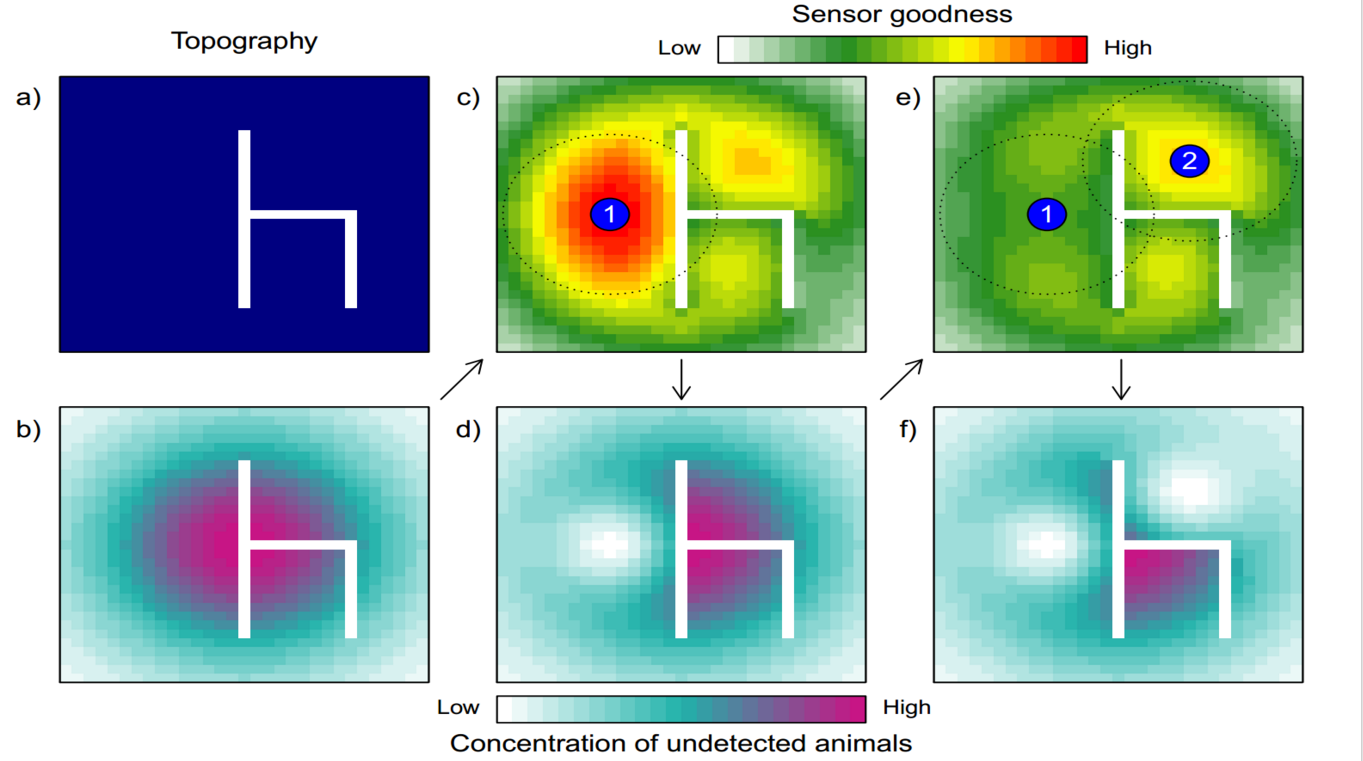
\includegraphics[scale=0.45]{suppression.png}
	\caption{An illustration of the Exact Suppression Algorithm.  In (a), we see a bathymetry grid with infinitely high walls (the white 'h' shape) on an otherwise flat plane (blue region).  In (b), we see Behavior Grid with a distribution (given by the OU movement model) of animals around the walls.  (c) shows the computed goodness of Sensor (receiver) locations within the study site.  The program first identifies location 1 (the blue circle) as having the highest unique data recovery rate, and places a receiver there.  The dotted lines represent the receiver's Detection Range.  In (d), the program suppresses the Behavior Grid by subtracting the ERT of each cell within Suppression Range.  Here the Suppression Range Factor is 1.0, so the Suppression Area is the same as the Detection Area).  In (e), the goodness grid is recalculated, taking into account the suppressed Behavior Grid.  Additionally, the program identifies location 2 as having the highest Unique Data Recovery Rate.  In (f), the Behavior Grid is again suppressed to account for the placement of receiver (2).}
\end{figure}

\subsection{Suppression Area}
As an input to the program, users can specify a Suppression Range Factor as a positive real number.  This factor is used to scale the Detection Range (Section~\ref{detectionRange}) and define a grid similar to the Detection Area (Section~\ref{detectionArea}).  The resulting grid is referred to as the Suppression Area.  The Suppression Area is centered over a receiver placement and cells within this area have their number of undetected transmissions reduced according to a Suppression Algorithm.  The suppression mechanic is used during the selection phase of the program.  After selecting each optimal receiver location (Section~\ref{selectionOfOptimalEmplacements}), the Suppression Area around that receiver location is suppressed.  The result of this mechanic is that emplacement selection is a sequential process, where selecting each emplacement depends upon the previous selection.  

\subsection{Suppression Algorithms}
\label{suppressionAlgorithms}
To promote the flexibility of our program, we provide users two algorithms for suppression.  The first offers a lower computation time at the cost of divergence from our theoretical model.  The second offers a higher fidelity model, but requires significantly more computation.

\subsubsection{Static Suppression}
\label{staticSuppression}
The Static Suppression algorithm takes a "cookie-cutter" approach and reduces the number of undetected transmissions in the Suppression Area by a user-specified factor (all cells within the Suppression Area are multiplied by a user-specified non-zero real number).  This computation is very simplistic, requiring only a scalar multiplication, and as such runs very quickly.  This is useful for simulations that intend to place a very large number of receivers.  The cost of this speed is that the algorithm ignores the attenuation and line of sight models completely.  For instance, a cell that is very far away from the receiver, and whose line of sight to the receiver is obstructed will be reduced by the same factor as a cell near the receiver with an unobstructed line of sight.  Obviously this is not a faithful representation of the conceptual models discussed earlier, but supplied as a computationally-simple alternative.

\subsubsection{Exact Suppression}
\label{exactSuppression}
The primary purpose of this algorithm was to discount exactly those transmissions which are likely to be observed by a placed receiver.  This algorithm uses the ERT given by the evaluation algorithms (the user-specified evaluation algorithm is used in both Goodness and Suppression calculations) to determine the number of transmissions to discount a cell by.  $ERT_{A,i,j}$ denotes the ERT in cell (i,j) observed from cell A.  Exact Suppression works first by computing $ERT_{A,i,j}$ for all cells (i,j)  within the Detection Area.  Then, each corresponding cell in the Behavior Grid, $B_{i,j}$, is reduced by $ERT_{A,i,j}$.  Finally, the goodness of all cells within Detection Range of a suppressed cell (all those that would have their goodness affected by the reduction) is recalculated.  Figure~\ref{suppressionImage} illustrates the Exact suppression algorithm.  

\section{Optimal Sensor Projection}
In normal research situations, users will have a set number of receivers to place within their study site.  The process of arriving at this number is likely unscientific, perhaps relying on user estimate (such as the user-perceived feasibility of receiving a given number of receivers).  Rather than guessing at the number of receivers to use, and hoping for an adequate data recovery rate, users should be able to calculate the marginal benefit (additional detections, increased Data Recovery Rates) of utilizing a variable number of receivers.   To this end, the program allows for the projected incremental benefit for a given number of additional receivers.  Our program facilitates this by allowing users to specify a number of receivers to project, returning graphs and metrics of the marginal increase in Data Recovery Rate.  With this data, users can determine an appropriate number of receivers to purchase, or construct an argument for purchasing more receivers.


\section{Time and Space Complexity}
\label{computationalComplexity}
To evaluate the temporal and spatial complexities of various elements of our program, we define the following variable inputs to the program:\newline
$n$ - The square root of the number of cells in the Bathymetry Grid, (the edge length of a square grid).  Also recall that the Bathymetry, Behavior, Goodness, and Coverage Grids are all of identical dimension, so $n$ roughly gives the edge dimensions of any of the afore mentioned Grids.\newline
$D_{range}$ - The Detection Range.  The square root of the number of cells in the Detection Grid (which is guaranteed to be a square).\newline
$k$ - The number of optimal placements to find.\newline

\subsection{Bathymetry Grid}
The bathymetry data for the study site is provided as a grid of $n^2$ cells.  This data must be copied into local memory (RAM), each cell in the grid takes O(1) time to copy, and O(1) space to hold.  Thus, the creation of the Bathymetry Grid will take O(1) * $n^2$ = O($n^2$) time and space..

\subsection{Behavior Grid}
Animal residency is computed as a function of the depth of a particular cell (Restricted Vertical Habitat), and the cell's location (OU/RW modeling).  This computation takes a constant [O(1)] amount of time.  The space required to store a single residency value for each of $n^2$ cells is also O(1).  Therefore, the population of the Behavior Grid takes O(1) * $n^2$ = O($n^2$) time and space.


\subsection{Line of Sight Computation}
\label{bigOLoS}
As discussed in Section~\ref{LoSAlgorithm}, the LoS algorithm is given as:\newline
1) Determine the intervening cells $C_{0...m}$ between $p$ and $q$\newline
2) Compute the slopes between $p$ and $C_i$ for all $i$ in $[0 ... m]$\newline
3) Choose the Critical Slope\newline
4) Project a line from $p$ to $q$ along the Critical Slope to find $D_{max}$.\newline

\textbf{Step 1} finds intervening cells by ray tracing, which can be done in linear ($O(n)$) time.  The number of cells considered ($n$), depends upon the distance between the receiver and the target cell\cite{rayTracing}.  Given that the Detection Grid has a radius of $D_{range}$, and that receivers are located in the center of the Detection Grid, the greatest distance between a receiver and a target cell in the Detection Grid occurs between a receiver and the corner cells of the Detection Grid (a distance of $\sqrt2*\frac{D_{range}}{2}$).  Thus, the number of cells considered when creating a list of intervening cells is $O(\sqrt2*\frac{D_{range}}{2})$ = $O(D_{range})$.

\textbf{Step 2} computes the slopes for each of the $m$ cells in $C$.  Computing the slope between two points takes $O(1)$ time to compute and space to store.  Therefore computing $m$ slopes takes $O(1)*O(m)=O(m)$ time and space.  As stated above, $m$ is at worst $O(D_{range})$ on the Detection Grid.  Thus, the slope computation is at worst $O(D_{range})$, requiring $O(D_{range})$ extra storage.

\textbf{Step 3} chooses the largest slope amongst all $m$ slopes.  Therefore, we must consider $m$ items, each requiring $O(1)$ time to consider as the largest.  Since, $m$ is $O(D_{range})$ on the Detection Grid, this step takes ($O(D_{range})$) time to compute, and $O(1)$ space to store.  

\textbf{Step 4} is a direct computation, requiring $O(1)$ time to compute and $O(1)$ space to store the result.

In total, the LoS computation time is $O(D_{range}) + O(1) + O(D_{range}) + O(1) = O(D_{range})$, requiring $O(D_{range}) + O(D_{range}) + O(1) + O(1) = O(D_{range})$ temporary storage space.
\begin{figure}[h]
	\label{rayTracingImg}
	\centering
	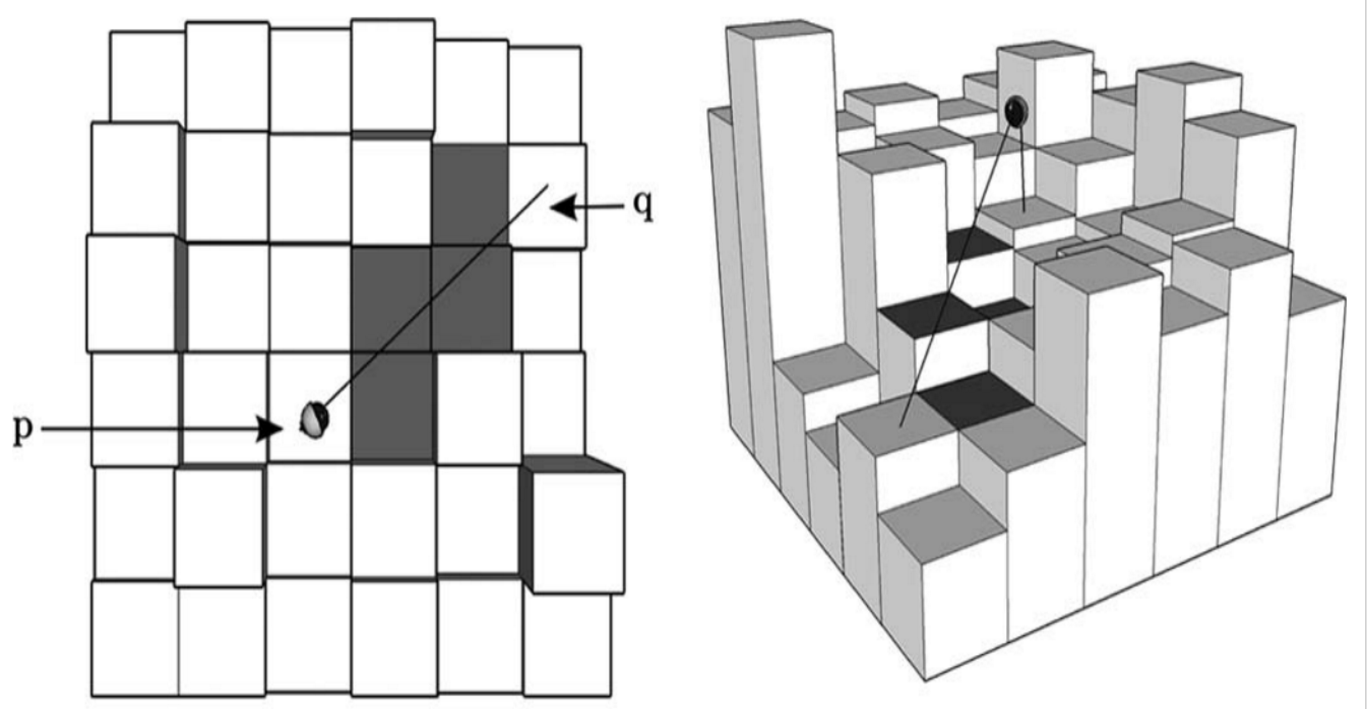
\includegraphics[scale=0.3]{rayTracing.png}
	\caption{An illustration of how ray tracing is used within a 3D environment to identify potential visual obstructions.  Ray tracing is used to determine which cells potentially block the line of sight between the receiver-contating cell $p$, and the target cell $q$.  Shaded cells must be evaluated by the Line of Sight algorithm to determine the portion of the water column in $q$ that is visible from $p$. \cite{Akbarzadeh2013}}
\end{figure}

\subsection{Goodness Grid}
Recall that the population of the Goodness Grid is performed by Evaluation Algorithms (Section~\ref{goodnessGrid}), each of which computes $ERT$ values for each of the $D_{range}^2$ cells in the Detection Grid.  These ERT values are then summed (requiring $O(D_{range}^2)$  time) to provide the Goodness value for a single cell of the $n^2$ cells in the Goodness Grid.  Thus, if we define the computational complexity of the ERT computation for Evaluation Algorithm $x$ to be $E_x$, the computational complexity for populating the entire Goodness Grid is is the time for ERT computation plus the time for  $O(n^2 * [D_{range}^2* E_x + D_{range}^2]) = O(n^2 * D_{range}^2 * [E_x + 1]) = O(n^2 * D_{range}^2 * E_x)$. 


\subsubsection{Evaluation Algorithm 1}
\label{bigObias1}
Section~\ref{bias1} gives the $ERT$ computation for Evaluation Algorithm 1 as:\newline
$ERT_{1,i,j} = B_{i,j} * P_{Attenuation}(Range(i,j))$

Accessing the value $ B_{i,j}$, finding the Range from i to j, and computing the attenuation due to range ($P_{Attenuation}(Range(i,j))$) and finding the product of the two can each be done in $O(1)$ time.  Thus, the ERT computation for this algorithm is $O(1) + O(1) + O(1) = O(1)$.  This computation will require $O(1)$ additional pieces of temporary storage for each intermediary value and the resulting product.


\subsubsection{Evaluation Algorithm 2 \& 3}
\label{bigObias23}
As discussed in Section~\ref{bias3}, the ERT computation for Evaluation Algorithms 2 and 3 is given as:\newline
$ERT_{2,i,j} =  B_{i,j} * P_{observation} * P_{Attenuation}(Range(i,j))$\newline

As mentioned in Section~\ref{bigObias1}, the product of $B_{i,j}$ and $P_{Attenuation}(Range(i,j))$ can be computed in $O(1)$ time with $O(1)$ temporary storage.  Computing the observable number of transmissions ($P_{observation}$) requires substantially more work.  Recall that we are using a 2-dimensional grid as the basis of our simulation and computing the third dimension as necessary by using a shape function.  Therefore, we first determine the deepest depth in each cell that can be seen by the receiver, and then use integration to compute the number of detectable transmissions ($P_{observation}$) within the visible part of the water column above that cell.  This leads us to the problem of finding the greatest depth (in each 2D cell) which is visible from the receiver.  We compute this via incremental ray tracing which can be done in  $O(D_{range})$ time.\cite{rayTracing}.  Then, using integration over the shape function, and known min/max visible depths, the total ($P_{observation}$) can be computed in $O(1)$ time.  Thus, the ERT computational complexity for this algorithm is $O(1) + O(1) + O(D_{range}) + O(1) = O(D_{range})$.  The algorithm will need to use $O(D_{range})$ temporary storage to compute Line of Sight, and $O(1)$ temporary space to store the resulting value.  Thus the total temporary storage required is given by $O(D_{range}+1)=O(D_{range})$.

%%\paragraph{Naive Method}
%%A naive solution to this question is to determine whether or not each cell in the three-dimensional grid can see the receiver.  Given that the volume of a sphere is $\frac{4/3}\pi r^{3}$, this solution would %%need to consider at least O($r^{3}$) cells, checking each for line of sight to the receiver.  As stated in Section~\ref{bigOLoS}, the time and space complexities of the LoS algorithm are both linear $O(r)$.  Thus, the time and space complexities for naively determining the line of sight to each cell in the Detection Grid are $O(r^3) * O(r) = O(r^4)$.  

\subsection{Optimal Receiver Placement}
The selection of the top $R_{opt}$ receiver locations requires the Goodness Grid to have been populated.  As previously stated, the selection process is iterative (requiring that suppression (if selected) be applied after each selection), as suppression causes goodness values to be altered.  The process of selecting a single receiver location is $O(n^2)$ since the algorithm must consider approximately $n^2$ possible receiver locations at each iteration.  After each location selection, suppression must be applied to the chosen location.  Due to the variability of the suppression algorithm, we use a variable  ($E_{suppression}$) to represent the expected runtime of the suppression algorithm.  Thus the computation time required for each selection-suppression step is $O(n^2 + E_{suppression})$.  The number of iterations required to run is given by the number of optimal ($R_{opt}$) and projected ($R_{proj}$) receiver placements requested.  In total, the runtime of the Optimal Receiver Placement step is $[R_{opt} + R_{proj}] * [O(n^2 + E_{suppression})] = O([R_{opt} + R_{proj}]* [n^2 + E_{suppression}])$.


\subsection{Suppression}
As discussed in Section~\ref{suppression}, the suppression mechanic is applied after the placement of a receiver.  The suppression mechanic has several options, each affecting the time and space complexity of the mechanism.  To better capture the complexity of the algorithms involved, we denote the following variables: \newline
$D_{range}$ - The Detection Range of a receiver.\newline
$d_{detection}$ - The edge size of the Detection Grid, equal to $2r+1$ cells.\newline
$f_{supp}$ - The Suppression Range Factor.  A positive real number. \newline
$r_{supp}$ - The Suppression Range. Equal to $f_{supp}*D_{range}$\newline
$d_{supp}$ - The square root of the number of cells in the Suppression Area.  The edge dimension of the Suppression Area.  Equal to $2*r_{supp} + 1$ cells.\newline

\subsubsection{Static Suppression Algorithm}
As stated in Section~\ref{staticSuppression}, the Static Suppression Algorithm multiplies all cells within the Suppression Area by a scalar constant.  This is a scalar multiplication that can be done in place, requiring $O(1)$ extra space, but requires a multiplication operation for each cell in the Suppression Area, which is $O(d_{supp} ^2) = O([2*f_{supp}*D_{range} + 1]^2) = O([4*f_{supp}^2*D_{range}^2 + 4*f_{supp}*D_{range} + 1]) = O(f_{supp}^2*D_{range}^2)$.  In most cases (excluding those where very sparse acoustic networks are desired), the Suppression Range Factor, $f_{supp}$, will be rather small (less than 2.0), which reduces the runtime complexity to $O(D_{range}^2)$.

\subsubsection{Exact Suppression}
As stated in Section~\ref{exactSuppression}, the Exact Suppression Algorithm uses the user-specified Evaluation Algorithm to calculate the number of transmissions that have already been observed and should be discounted from future consideration.  We define $E_{x}$ to denote the expected runtime for Evaluation Algorithm x's computation of a single cell's ERT.  We also define $T_{x}$ to denote the expected temporary storage requirement for Evaluation Algorithm x single-cell ERT computation.  The Exact Suppression Algorithm is broken into three distinct steps: Suppression Area ERT computation, Behavior Grid Updtate, and Goodness Grid Recalculation.
\newline

\textbf{Suppression Area ERT Computation}\newline
The suppression algorithm first determines the ERT for each cell within the Suppression Area, and stores them in the ERT Area, a temporary Grid with the same dimension as the Suppression Area.  This step is similar to the Evaluation process, with the exception that the Suppression Area's dimensions differ from those of the Detection Grid by a factor of $f_{supp}$ (the Suppression Area is usually larger than the Detection Grid).  The computation of the ERT Area requires $E_{x}$ time and  $T_x$ temporary space for each of the $d_{supp}^2$ cells in the Suppression Area.  An additional  $O(1)$ temporary space will also be needed to store the resulting ERT values.  Therefore, the ERT computation will require $O(E_{x} * d_{supp}^2)$ time and $O((1 + T_x)* d_{supp}^2) = O(d_{supp}^2 * T_x)$ temporary storage.

\textbf{Behavior Grid Update}\newline
Next, the suppression algorithm subtracts the ERT Area from the corresponding area in the Behavior Grid.  This is a simple subtraction operation over each corresponding cell in the grids.  Because each subtraction takes $O(1)$ time and temporary storage, the time and space complexities are both given by $O(1) * O(d_{supp}^2) = O(d_{supp}^2)$.

\textbf{Goodness Grid Recalculation}\newline
Finally, the goodness values of all cells within Detection Range of the Suppression Area must have their Goodness value updated (as we have just reduced the ERT of one or more cells within their Detection Grid).  The area affected by suppression, and therefore requiring recalculation, is a square with edge diameter $2 * (d_{supp} + D_{range}) + 1$.  Each cell in this area will require  $O(D_{range}^2 * E_x)$ time to compute.  The total time for updating the Goodness Grid is then: $O([2 * (d_{supp} + D_{range}) + 1]^2 * O(D_{range}^2 * E_x)) = O((d_{supp} + D_{range})^2 + D_{range}^2 * E_x)$.  The Goodness Grid update will require $D_{range}^2 * (T_x + 1) = O(D_{range}^2 * T_x)$ temporary storage to compute and store intermediate ERT values.  This temporary storage can be recycled for each sequential Goodness Cell computation.


The total computation time for the Exact Suppression Algorithm is then given by O(ERT Computation) + O(Behavior Grid Update) + O(Goodness Grid Recalculation). This is a total of $O(E_{x} * d_{supp}^2) + O(d_{supp}^2) + O((d_{supp} + D_{range})^2 + D_{range}^2 * E_x)$ time.  The algorithm will also require $O(MAX(d_{supp}^2 , D_{range}^2) * T_x)$ temporary storage, which can be recycled between each of the above stages.

%%TODO rayTracing multiply defined (webpage and document) check refs
